\chapter{Solutions}
\label{ch:solutions}

In programming there nearly always exist multiple ways to solve a
problem. Your code does not have to be exactly the same as the
solutions given in this chapter. Occasionally some of these solutions
include \texttt{R} functions and optional arguments that have not
already been introduced before. These additional `bells and whistles'
are optional, and the code will still work without them. Several
exercises depend on the \texttt{geostats} package, which we assume to
have been loaded into memory:

\begin{console}
library(geostats)
\end{console}
  
\section{The basics}
\label{sec:sol-basics}

\begin{enumerate}
\item Plotting the sine:

\begin{script}
theta <- seq(from=0,to=2*pi,length.out=50)
plot(theta,sin(theta),type='l')
\end{script}

Adding the cosine:

\begin{script}[firstnumber=3]
lines(theta,cos(theta),lty=2)
\end{script}

\noindent where \texttt{lty=2} creates a dashed line (see
\texttt{?par}).

\item Define the function

\begin{script}
ellipse <- function(a=1,b=1,alpha=pi/4){
  beta <- seq(from=0,to=2*pi,length.out=50)
  x <- a*cos(alpha)*cos(beta) - b*sin(alpha)*sin(beta)
  y <- a*sin(alpha)*cos(beta) + b*cos(alpha)*sin(beta)
  plot(x,y,type='l',asp=1)
}
\end{script}

Using the new function:

\begin{console}
> ellipse() # produces a circle
> ellipse(a=1,b=2)
\end{console}
    
\item Here we need a conditional statement:

\begin{script}
multiples <- function(n,m){
  remainder <- max(n,m) %% min(n,m)
  if (remainder == 0){
    decision <- paste(n,'and',m,'are multiples')
  } else {
    decision <- paste(n,'and',m,'are not multiples')
  }
  print(decision)
}
\end{script}

\noindent where the \texttt{paste} function concatenates text strings
(see \texttt{?paste} for details).

\item This exercise requires a for-loop:
  
\begin{script}
triangle <- function(n){
  for (i in 1:n){
    print(rep(i,i))
  }
}
\end{script}
  
\end{enumerate}

\section{Plotting data}
\label{sec:sol-plotting}

\begin{enumerate}

\item The bars produced by \texttt{barplot} correspond to years,
  whereas those produced by \texttt{hist} correspond to the number of
  earthquakes per year. The following code shows both diagrams side by
  side:
  
\begin{script}
data(declustered,package='geostats')
quakesperyear <- countQuakes(declustered,minmag=4.5,from=2000,to=2016)
par(mfrow=c(1,2))
barplot(quakesperyear)
hist(quakesperyear)
\end{script}

\item\label{it:ABsol} Write a plotting function to avoid duplicate
  code:

\begin{script}
rugdensity <- function(dat){
  plot(density(dat))
  rug(dat)
}
\end{script}

Then we can use this function to show that the (reciprocal) ratios of
random numbers drawn from a symmetric (e.g. uniform) distribution
follow a skewed distribution:

\begin{script}[firstnumber=5]
A <- runif(100)
B <- runif(100)
par(mfrow=c(2,2))
rugdensity(A/B)
rugdensity(B/A)
rugdensity(log(A/B))
rugdensity(log(B/A))
\end{script}

\item\label{it:xyrandsol} Using the optional \texttt{min} and
  \texttt{max} arguments of the \texttt{runif($\ldots$)} function:

\begin{script}
library(MASS)
x <- runif(1000,min=-1,max=1)
y <- runif(1000,min=2,max=22)
contour(kde2d(x,y))
points(x,y)
\end{script}

\item Continuing the previous solution:

\begin{script}[firstnumber=6]
par(mfrow=c(1,2))
cdfx <- ecdf(x)
plot(cdfx)
cdfy <- ecdf(y)
plot(cdfy)
\end{script}

Querying the ECDFs:

\begin{console}
> cdfx(0)
[1] 0.492
> cdfy(c(7,17))
[1] 0.248 0.748
\end{console}

You may get slightly different values due to the randomness of the
\texttt{runif($\ldots$)} function. But they should hover around
$\sim{0.5}, \sim{0.25}$ and $\sim{0.75}$, respectively.

\end{enumerate}
  
\section{Summary statistics}
\label{sec:sol-summary-statistics}

\begin{enumerate}
\item Carrying on from Section~\ref{sec:R-plotting}.\ref{it:anscombe},
  and using a for-loop to avoid duplicate code:

\begin{script}
nc <- ncol(anscombe)                  # number of columns
mv <- matrix(0,nrow=2,ncol=nc)        # mv = 'mean-variance'
rownames(mv) <- c('mean','variance')
colnames(mv) <- colnames(anscombe)
for (i in 1:nc){                      # loop through the columns
  mv['mean',i] <- mean(anscombe[,i])
  mv['variance',i] <- var(anscombe[,i])
}
\end{script}

Querying the result and rounding to two significant digits:

\begin{console}
> signif(mv,2)
         x1 x2 x3 x4  y1  y2  y3  y4
mean      9  9  9  9 7.5 7.5 7.5 7.5
variance 11 11 11 11 4.1 4.1 4.1 4.1
\end{console}

\item First define a function to generate $n$ random numbers and
  average them:

\begin{script}
meanofmeans <- function(n=10,N=100){
  m <- rep(0,N)            # initialise
  for (i in 1:N){
    m[i] <- mean(runif(n)) # populate
  }
  c(mean(m),sd(m))         # return the results
}
\end{script}

An equivalent but faster solution would be to replace the for-loop
with:

\begin{script}[firstnumber=3]
  R <- runif(n*N)
  M <- matrix(R,nrow=n,ncol=N)
  m <- colMeans(M)
\end{script}

Now apply the \texttt{meanofmeans} function to $n=10, 100, 1000$ and
$10000$, and store the results in a matrix:

\begin{script}[firstnumber=8]
n <- c(10,100,1000,10000)       # Initialise
mom <- matrix(0,length(n),2)    # the
colnames(mom) <- c('mean','sd') # results
rownames(mom) <- n              # matrix.
for (i in 1:length(n)){         # Fill
  mom[i,] <- meanofmeans(n[i])  # the
}                               # matrix.
\end{script}

Check the result at the command prompt and verify that the mean
converges to 0.5, and the standard deviation gets ever smaller with
increasing $n$:

\begin{console}
> signif(mom,4)
        mean       sd
10    0.4977 0.092320
100   0.5033 0.025540
1000  0.5003 0.009316
10000 0.5002 0.002923
\end{console}
  
Again, results may vary slightly between runs. The sample size
dependency of the mean of means is further investigated in
Chapter~\ref{sec:stderr}.

\item Filling the vector of 500 counts using a for-loop:

\begin{script}
N <- 500
counts <- rep(0,N)
for (i in 1:N){
  r <- runif(1000,max=200)
  counts[i] <- sum(r < 1)
}
\end{script}

Alternatively, we can also solve the problem more quickly without a
for-loop:

\begin{script}
n <- 1000
N <- 500
r <- runif(n*N,max=200)
m <- matrix(r,nrow=n,ncol=N)
counts <- colSums(m<1)
\end{script}

You should see that the mean approximately equals the variance:

\begin{console}
> mean(counts)
[1] 4.928
> var(counts)
[1] 5.01685
\end{console}

This phenomenon is further explored in Chapter~\ref{ch:poisson}.

\item Taking the logratio of two matrices of random numbers:

\begin{script}
n <- 100
N <- 10
A <- matrix(runif(n*N),nrow=n,ncol=N)
B <- matrix(runif(n*N),nrow=n,ncol=N)
boxplot(log(A/B))
\end{script}

You should get ten broadly similar looking box plots.

\end{enumerate}

\section{Probability}
\label{sec:sol-probability}

\begin{enumerate}
  
\item An IGSN consists of two parts. The first part consists of up to
  five letters.  There 26 possible one-letter combinations, $26^2$
  possible two-letter combinations etc. Therefore, the total number of
  lab identifiers is $\sum_{i=1}^526^i=12,356,630$. The second part
  consists of four letters (A--Z) or numbers (0--9). The total number
  of possibilities for these is $36^4=1,679,616$. Therefore, the total
  number of possible IGSNs is

\begin{console}
> sum(26^{1:5}) * 36^4
[1] 2.075439e+13
\end{console}

\item There are $\binom{20}{5}$ choices for the first group,
  $\binom{15}{5}$ for the second, $\binom{10}{5}$ for the third and
  $\binom{5}{5}$ for the fourth. Hence the total number of
  combinations is:

\begin{console}
> i <- seq(from=5,to=20,by=5)
> prod(choose(i,5))
[1] 11732745024
\end{console}

\item Let $A$, $B$ and $C$ stand for for andesite, basalt and
  carbonate, respectively, and let $p_A$, $p_B$ and $p_C$ be their
  respective probabilities in the population (i.e. $p_A=0.3$,
  $p_B=0.2$ and $p_C=0.5$). The probability that none of $n$ clasts
  are made of andesite is $(1-p_A)^n$. So we might think that the
  probability of missing at least one clast type is:
  \[
  p(\mbox{no~}A, B \mbox{~or~}C) \overset{?}{=}
  (1-p_A)^n + (1-p_B)^n + (1-p_C)^n
  \]
  
  However this would double-count the instances where two clast types
  are missing. For example, if a sample of $n$ clasts does not contain
  any basalt or carbonate, then this means that it contains only
  andesite.  The probability that this happens is $p_A^n$. Similarly,
  the probabilility of missing both andesite and carbonate is $p_B^n$,
  and the probability of missing both andesite and basalt is $p_C^n$.
  Removing these double-counted events:
  \[
  p(\mbox{no~}A, B \mbox{~or~}C) =
  (1-p_A)^n + (1-p_B)^n + (1-p_C)^n - p_A^n - p_B^n - p_C^n
  \]

  Implementing this expression in \texttt{R}:
\begin{script}
ABC <- function(n,pA,pB,pC){
  if (n<3){   # samples of fewer than 3 clasts
    p <- 0    # are definitely incomplete
  } else {
    p <- (1-pA)^n + (1-pB)^n + (1-pC)^n - pA^n - pB^n - pC^n
  }
  return(1-p)
}
\end{script}


Evaluating the \texttt{ABC} function at the command line for different
values of $n$:

\begin{console}
> ABC(n=10,pA=0.3,pB=0.2,pC=0.5)
[1] 0.8634136
> ABC(n=20,pA=0.3,pB=0.2,pC=0.5)
[1] 0.9876719
> ABC(n=14,pA=0.3,pB=0.2,pC=0.5)
[1] 0.9491764
\end{console}

In conclusion we need to collect at least 14 clasts to have 95\%
certainty that all lithologies are represented in our sample.

\item Using Equation~\ref{eq:totalBayes}:
  \[
  \begin{split}
    p(\mbox{Fe}|\mbox{anomaly}) & =
    \frac{p(\mbox{anomaly}|\mbox{Fe}) p(\mbox{Fe})}
         {p(\mbox{anomaly}|\mbox{Fe}) p(\mbox{Fe}) +
           p(\mbox{anomaly}|\mbox{Cr}) p(\mbox{Cr}) +
           p(\mbox{anomaly}|\mbox{other}) p(\mbox{other})} \\
         & = \frac{0.95 \times 0.001}
         {(0.95 \times 0.001) + (0.98 \times 0.0005) +
          (0.01 \times 0.9985)
         } = 0.083 = 8.3\% \\
    p(\mbox{Cr}|\mbox{anomaly}) & =
    \frac{p(\mbox{anomaly}|\mbox{Cr}) p(\mbox{Cr})}
         {p(\mbox{anomaly}|\mbox{Fe}) p(\mbox{Fe}) +
           p(\mbox{anomaly}|\mbox{Cr}) p(\mbox{Cr}) +
           p(\mbox{anomaly}|\mbox{other}) p(\mbox{other})} \\
         & = \frac{0.98 \times 0.0005}
         {(0.95 \times 0.001) + (0.98 \times 0.0005) +
          (0.01 \times 0.9985)
         } = 0.043 = 4.3\%
  \end{split}
  \]

  Hence the probability that the magnetic anomaly is caused by an ore
  deposit is $8.3+4.3=12.6$\%.
  
\end{enumerate}
  
\section{The binomial distribution}
\label{sec:sol-binomial}

\begin{enumerate}

\item Let $p(A)$ and $p(N)$ be the probability of counting an arboreal
  and non-arboreal pollen, respectively (where $p(A)+p(N)=1$). Then:

  \[
  \frac{p(A)}{p(N)} = 4 = \frac{p(A)}{1-p(A)}
  \Rightarrow p(A) = \frac{4}{1+4} = 0.8
  \]

  So if $n=20$, then the most likely outcome is $20\times{0.8}=16$
  arboreal and $20\times{(1-0.8)}=4$ non-arboreal pollen. Using the
  same calculation, an arboreal/non-arboreal count ratio of 9 would
  correspond to a probability $p(A)=9/10=0.9$, which would lead to an
  outcome of $20\times{0.9}=18$ arboreal and $20\times{(1-0.9)}=2$
  non-arboreal pollen. The probability of observing an outcome at
  least as extreme as this is given by:

\begin{console}
> 1-pbinom(q=17,size=20,prob=0.8)
[1] 0.2060847
\end{console}

or, equivalently:

\begin{console}
> pbinom(q=17,size=20,prob=0.2,lower.tail=FALSE)
> pbinom(q=2,size=20,prob=0.2)
\end{console}

In conclusion, there is a 20\% chance of observing an $A/N$ count
ratio of greater or equal than 9 when the actual population ratio
is~4.
  
\item To answer the first question, we formulate a two-sided
  hypothesis:

  $H_\circ: p(\mbox{female}) = p(\mbox{male})$\\
  $H_a: p(\mbox{female}) \neq p(\mbox{male})$

  Then the 2.5 and 97.5 percentiles of the binomial null distribution
  are given by:

\begin{console}
> qbinom(p=c(0.025,0.975),size=50,prob=0.5)
[1] 18 32
\end{console}

So the rejection is $R=\{0,\ldots,17,33,\ldots,50\}$, which does not
include the observed outcome of 32 male fossils. Equivalently, using
the \texttt{binom.test} function:
  
\begin{console}
> h <- binom.test(x=32,n=50,p=0.5,alternative="two.sided")
> h$p.value
[1] 0.06490865
\end{console}

$0.06490865>0.05$ and therefore the two-sided hypothesis is not
rejected. To answer the second question, we carry out a one-sided
hypothesis test:

  $H_\circ: p(\mbox{female}) = p(\mbox{male})$\\
  $H_a: p(\mbox{female}) > p(\mbox{male})$

\noindent whose 95 percentile is given by:

\begin{console}
> qbinom(p=0.95,size=50,prob=0.5)
[1] 31
\end{console}

This leads to a rejection region of $R=\{32,\ldots,50\}$, which
includes the outcome of 32 female fossils. Hence the one sided
hypothesis is rejected. Equivalently:

\begin{console}
> h <- binom.test(x=32,n=50,p=0.5,alternative="greater")
> h$p.value
[1] 0.03245432
\end{console}

\noindent which is half of the one-sided p-value and less than
0.05. The one-sided hypothesis is more powerful than the two-sided
version, leading to rejection of $H_\circ$. Thus the one-sided and
two-sided hypothesis tests lead to different conclusions for the same
dataset. It is important that the test is chosen before the experiment
is completed. So you must decide on your scientific question before
designing your study. In the dinosaur example, it would be bad
practice to decide on a one-sided hypothesis test \emph{after} seeing
that female fossils are more abundant in the bone bed than male ones.

\item This exercise is all about type-I errors. Using \texttt{rbinom}
  to generate the synthetic data:

\begin{script}
type1test <- function(p=0.2,n=50,N=100){
  r <- rbinom(n=n,size=N,prob=p)
  pval <- rep(0,n)
  for (i in 1:n){
    h <- binom.test(x=r[i],n=N,p=p)
    pval[i] <- h$p.value
  }
  sum(pval<0.05)
}
\end{script}

The function is to be used like this:

\begin{console}
> type1test()
[1] 2
> type1test()
[1] 3
> type1test()
[1] 0
\end{console}

You get a different result every time because \texttt{rbinom}
generates a different set of numbers every time. The number of
rejected null hypotheses should hover around 5\%.  Therefore we would
expect that, on average, 2.5 out of every 50 tests should fail.

\item\label{it:binomtest} The 95\% confidence interval for $p(A)$ is
  given by:

\begin{console}
> binom.test(x=12,n=20)$conf.int
[1] 0.3605426 0.8088099
\end{console}

Note that we are not really using \texttt{binom.test} to carry out a
hypothesis test. We are only interested in the confidence interval.
The lower value of the confidence interval for $p(A)=0.3605426$
corresponds to an $A/N$-ratio of

\[
\frac{p(A)}{p(N)} = \frac{p(A)}{1-p(A)} =
\frac{0.3605426}{1-0.3605426} = 0.5638258
\]

A value of $p(A)=0.8088099$ corresponds to an $A/N$-ratio of

\[
\frac{p(A)}{p(N)} = \frac{p(A)}{1-p(A)} =
\frac{0.8088099}{1-0.8088099} = 4.230396
\]

Hence the 95\% confidence interval for $A/N$ is
$(0.5638258,4.230396)$.

\end{enumerate}
  
\section{The Poisson distribution}
\label{sec:sol-poisson}

\begin{enumerate}
\item If one magnitude $\geq{9}$ event happens every 13.5 years, then
  this means that there is a $\lambda=1/13.5$ chance that one event
  will happen next year, and the chance that exactly two such events
  happen is given by Equation~\ref{eq:poispmf}:

  \[
  P\left(k=2|\lambda=\frac{1}{13.5}\right) = \frac{\lambda^k
    e^{-\lambda}}{k!} = \frac{\exp\left[-\frac{1}{13.5}\right]}{13.5^22!} =
  0.00255 ~ (0.255\%)
  \]

  In \texttt{R}:

\begin{console}
> dpois(x=2,lambda=1/13.5)
[1] 0.002547607
\end{console}

The number of magnitude $\geq{9}$ earthquakes per century is
$\lambda={100/13.5}$. The chance that no such earthquake will happen
during the next century is:

  \[
  P\left(k=0|\lambda=\frac{100}{13.5}\right) =
  \exp\left[{-\frac{100}{13.5}}\right] =
  0.000607 (0.0607\%)
  \]

\item The expected number of fission tracks is

  \[
  (1\times{10}^{6}\mbox{yr})
  \times
  \left(\frac{{8.46}\times{10}^{-17}}{\mbox{atoms}\cdot\mbox{yr}}\right)
  \times({6.022}\times{10}^{10}\mbox{atoms})=50.95
  \]

  The probability that the crystal contains fewer
  than 50 fission tracks is:

\begin{console}
> L <- 1e6 * 8.46e-17 * 6.022e11
> ppois(q=50,lambda=L)
[1] 0.4843836
\end{console}

The probability that it contains between 40 and 60 fission tracks is:

\begin{console}
> ppois(q=60,lambda=L) - ppois(q=40,lambda=L)
[1] 0.8393979
\end{console}

\item This problem requires a one-sided hypothesis test:

  $H_\circ: \lambda=2$\\
  $H_a: \lambda<2$\\

  In \texttt{R}:

\begin{console}
> h <- poisson.test(x=12,T=10,r=2,alternative='less')
> h$p.value
[1] 0.03901199
\end{console}

$H_\circ$ is rejected on a 95\% confidence level, and so it would be
best to cease operations and abandon the mining site.

\item To construct a 95\% confidence interval, we again use
  \texttt{poisson.test}, but have no need to formulate a null
  hypothesis. This is similar to
  exercise~\ref{sec:sol-binomial}.\ref{it:binomtest}:

\begin{console}
> h <- poisson.test(x=30,T=10)
> h$conf.int
[1] 2.024087 4.282687
\end{console}

The profitability cutoff of 2 diamonds per tonne falls below this
confidence interval. So we can conclude that the second site is
profitable.

\end{enumerate}

\section{The normal distribution}
\label{sec:sol-gauss}

\begin{enumerate}

\item This is an illustration of the central limit theorem. Here is a
  solution that does not require a for loop:

\begin{script}
# np = the number of Poisson values per sum
# ns = the number of sums
CLT <- function(np=100,ns=200){
  r <- rpois(n=np*ns,lambda=1.2)   # create all random numbers at once
  mat <- matrix(r,nrow=np,ncol=ns) # put the values in one big matrix
  sums <- colSums(mat)  # take the column sums (instead of a for loop)
  hist(sums)            # plot the histogram
  mu <- mean(sums)      # compute the mean
  sigma <- sd(sums)     # compute the standard deviation
  proximal <- sums>(mu-2*sigma) & sums<(mu+2*sigma) # logical vector
  return(sum(proximal)/ns)         # returns a value between 0 and 1
}
\end{script}

Running this script from the console should return a value of
approximately 0.95:

\begin{console}
> CLT()
[1] 0.955
\end{console}

Results will vary slightly due to the randomness of \texttt{rpois}.

\item The probability that someone has an IQ of less than 90 is

\begin{console}
> pnorm(q=90,mean=100,sd=15)
[1] 0.2524925
\end{console}

The probability that someone has an IQ of more than 120 is

\begin{console}
> pnorm(q=120,mean=100,sd=15,lower.tail=FALSE)
[1] 0.09121122
\end{console}

The probability that two such people are paired up is the product
of these two values, which is 2.3\%.
  
\item The probability that the height of an American male exceeds
  72 inches is

\begin{console}
> pnorm(q=72,mean=69.3,sd=2.8,lower.tail=FALSE)
[1] 0.1674514
\end{console}

The probability that an American female is more than 72 inches tall is

\begin{console}
> pnorm(q=72,mean=64,sd=2.8,lower.tail=FALSE)
[1] 0.002137367
\end{console}

The sum of these two values is 17.0\%. The 90 percentile for men is

\begin{console}
> p90 <- qnorm(p=0.9,mean=69.3,sd=2.8)
> p90
[1] 72.88834
\end{console}

The fraction of women who exceed this height is

\begin{console}
> pnorm(q=p90,mean=64,sd=2.8,lower.tail=FALSE)
[1] 0.0007507106
\end{console}

\noindent which is 0.075\%.

\item Here we need to evaluate the bivariate normal likelihood
  (equation~\ref{eq:2dgauss}). Unfortunately, this function is not
  part of base \texttt{R} so we need to implement it ourselves:

\begin{script}
dmvnorm <- function(vec,mu=rep(0,2),sigma=matrix(1,nrow=2,ncol=2)){
  num <- exp(0.5 * t(vec - mu) %*% solve(sigma) %*% (vec - mu))
  den <- 2*pi*sqrt(det(sigma))
  return(num/den)
}
\end{script}

Using these data to evaluate the bivariate normal densities of $X$ and
$Y$:

\begin{script}[firstnumber=6]
muX <- c(1,2)
muY <- c(3,4)
SigmaX <- matrix(c(1,-1,-1,3),nrow=2,ncol=2)
SigmaY <- matrix(c(2,2,2,7),nrow=2,ncol=2)
X <- c(2,1)
Y <- c(5,7)
dX <- dmvnorm(X,mu=muX,sigma=SigmaX)
dY <- dmvnorm(Y,mu=muY,sigma=SigmaY)
\end{script}

\noindent which produces the following output:

\begin{console}
> dX
[1,] 0.1855463
> dY
[1,] 0.1511973
\end{console}

So outcome $X$ is more likely than outcome $Y$. 

\end{enumerate}

\section{Error propagation}
\label{sec:sol-errorprop}

\begin{enumerate}
\item Let $x$ be the height difference between points A and B
  ($x=25\pm0.25$~m), and let $y$ be the height difference between B
  and C ($y=50\pm0.5$~m). Then the height difference between A and C
  is simply $z=x+y=75$~m. To propagate the uncertainty of this
  estimate, we use Equation~\ref{eq:addition} with $a=0$ and $b=c=1$:

  \[
  s[z]^2 = s[x]^2 + s[y]^2 = 0.25^2 + 0.5^2 = 0.3125
  \Rightarrow s[z] = \sqrt{0.3125} = 0.559017
  \]

  Note that the uncertainty of both $x$ and $y$ is 1\%, but the
  uncertainty of $z$ is only 0.75\%.

\item \begin{enumerate}

\item Density is mass divided by volume, hence $\mbox{density}(A) =
  105/36 = 2.92$~g/cm\textsuperscript{3} and $\mbox{density}(B) =
  30/10 = 3.00$~g/cm\textsuperscript{3}.

\item The uncertainty is calculated with the formula for a quotient
  (equation~\ref{eq:division}):
\[
\left(\frac{s[z]}{z}\right)^2 = \left(\frac{s[x]}{x}\right)^2 +
    \left(\frac{s[y]}{y}\right)^2
\]
\noindent where $z$ is density, $x$ is mass and $y$ is volume. Thus
$s[\mbox{density}(A)] =
\frac{105}{36}\sqrt{\left(\frac{2}{105}\right)^2+\left(\frac{0.15}{36}\right)^2}=0.057$~g/cm\textsuperscript{3}
and $s[\mbox{density}(B)] =
\frac{30}{10}\sqrt{\left(\frac{2.5}{30}\right)^2+\left(\frac{0.4}{10}\right)^2}=0.277$~g/cm\textsuperscript{3}.
\item The 95\% confidence intervals for the two densities are
  approximately 2$\times$ their standard deviations. So for sample A,
  the 95\% confidence interval is
  2.92$\pm$0.11~g/cm\textsuperscript{3}, and for sample B it is
  3.00$\pm$0.55~g/cm\textsuperscript{3}.
\item The confidence interval for density($A$) overlaps with
  density(B) and vice versa. Therefore, we cannot rule out the
  possibility that the true densities are equal.
\end{enumerate}

\item The formula for the size shift does not directly fit into any of
  the equations of Section~\ref{sec:errorpropexamples}. Therefore we
  have to apply the chain rule:
  \[
  \begin{split}
    x & = \rho_z-1 = 3.85 \mbox{~and~} y = \rho_q-1 = 1.65 \\
    z & = \frac{x}{y} = \frac{3.85}{2.65} = 2.333\\
    SS & = a \ln\left(z\right) = \frac{1}{0.69}\ln(2.33) = 1.228
  \end{split}
  \]
  Following the same steps for the error propagation:
  \[
  \begin{split}
    s[x] & = s[\rho_z] = 0.10 \mbox{~and~} s[y] = s[\rho_q] = 0.05 \mbox{~(using
      Equation~\ref{eq:subtraction})}\\
    s[z] & = z\sqrt{\left(\frac{s[x]}{x}\right)^2+\left(\frac{s[y]}{y}\right)^2}
    = \frac{3.85}{2.65}\sqrt{\left(\frac{0.10}{3.85}\right)^2+\left(\frac{0.05}{2.65}\right)^2}
    = 0.047 \mbox{~(using Equation~\ref{eq:division})}\\
    s[SS] & = a\frac{s[z]}{z} = \frac{1}{0.69}\frac{0.047}{2.333} = 0.029
    \mbox{~(using Equation~\ref{eq:logarithms})}
  \end{split}
  \]

\item \begin{enumerate}
\item Calculating the means:

\begin{script}
K40 <- c(2093,2105,2055,2099,2030)
Ar40 <- c(6.015,6.010,6.030,6.005,6.020,6.018)
meanK40 <- mean(K40)
meanAr40 <- mean(Ar40)
\end{script}

\item The standard errors of the means:

\begin{script}[firstnumber=5]
nK40 <- length(K40)
nAr40 <- length(Ar40)
seK40 <- sd(K40)/sqrt(nK40)
seAr40 <- sd(Ar40)/sqrt(nAr40)
\end{script}

\item The $^{40}$Ar/$^{40}$K-ratio and its standard error, propagated
  using Equation~\ref{eq:division}:

\begin{script}[firstnumber=9]
Ar40K40 <- meanAr40/meanK40
seAr40K40 <- Ar40K40*sqrt((seAr40/meanAr40)^2+(seK40/meanK40)^2)
\end{script}

\item Calculating the K--Ar age:

\begin{script}[firstnumber=11]
L <- 5.543e-4 # lambda
LLe <- 9.3284 # lambda/lambda_e
age <- log(1+LLe*Ar40K40)/L
\end{script}

Propagating its uncertainty requires breaking down the calculation
into two steps:

\[
\begin{split}
  z & = 1 + \frac{\lambda}{\lambda_e}\left(\frac{^{40}Ar }{^{40}K}\right)
    \mbox{~(which can be propagated using Equation~\ref{eq:addition})}\\
  \mbox{and~}t & = \frac{1}{\lambda}\ln(z) 
  \mbox{~(which can be propagated using Equation~\ref{eq:logarithms})}
\end{split}
\]

In \texttt{R}:

\begin{script}[firstnumber=14]
z <- 1+LLe*Ar40K40
sez <- LLe*seAr40K40 # using equation 8.10
se_age <- sez/(L*z)  # using equation 8.15
\end{script}

Running this script in \texttt{R} yields

\begin{console}
> age
[1] 48.11483
> se_age
[1] 0.3331236
\end{console}
  
\end{enumerate}

\end{enumerate}
  
\section{Comparing distributions}
\label{sec:sol-comparingdistributions}

\begin{enumerate}

\item This is an application of \texttt{R}'s \texttt{chisq.test}
  function. First we amalgamate the data columns with the fewest
  counts. Then we apply a two-sample chi-square test to this new
  table:

\begin{script}
data(forams,package='geostats')
abundant <- forams[,c('quinqueloba','pachyderma','incompta',
                      'glutinata','bulloides')]
other <- rowSums(forams[,c('uvula','scitula')])
dat <- cbind(abundant,other)
h <- chisq.test(dat)
\end{script}

Probing the outcome of these calculations:

\begin{console}
> h$p.value
[1] 0.7977184
\end{console}

Hence there is insufficient evidence to prove that the two samples
reflect different ecosystems.

\item Using Equation~\ref{eq:tci}:

\begin{script}
data(pH,package='geostats')      # load the data
n <- length(pH)                  # sample size
mu <- mean(pH)                   # arithmetic mean
se <- sd(pH)/sqrt(n)             # standard error of the mean 
tfact <- qt(p=0.025,df=n-1)      # t(df,alpha/2)
ci <- mu + c(tfact*se,-tfact*se) # confidence interval
\end{script}

\noindent which produces

\begin{console}
> ci
[1] 4.671497 5.298503
\end{console}

\item Comparing the t-test and Wilcoxon test:

\begin{script}
A <- seq(from=0,to=8,by=2)
B <- seq(from=3,to=15,by=2)
ht <- t.test(A,B)
hw <- wilcox.test(A,B)
\end{script}

\noindent which produces the following outcomes:

\begin{console}
> ht$p.value
[1] 0.04325446
> hw$p.value
[1] 0.07323232
\end{console}

The null hypothesis is rejected by the t-test but not by the Wilcoxon
test. This is representative of a general tendency for non-parametric
hypothesis tests to be less powerful than their parametric
counterparts.
  
\item\label{it:sol-DZ-MDS} There are 13 samples in the \texttt{DZ},
  whose Kolmogorov-Smirnov statistics can be evaluated in a double for
  loop.

\begin{script}
data(DZ,package='geostats') # load the data
ns <- length(DZ)            # number of samples
maxKS <- 0                  # initialise the least similar K-S value
minKS <- 1                  # initialise the most similar K-S value
for (i in 1:(ns-1)){        # loop through the rows
  for (j in (i+1):ns){      # loop through the columns
    KS <- ks.test(DZ[[i]],DZ[[j]])$statistic
    if (KS < minKS){
      minKS <- KS           # update the least similar K-S values
      mostsimilar <- c(i,j)
    }
    if (KS > maxKS){
      maxKS <- KS           # update the most similar K-S values
      leastsimilar <- c(i,j)
    }
  }
}
\end{script}

Plotting the most similar and least similar pairs as Q-Q plots:

\begin{script}[firstnumber=18]
par(mfrow=c(1,2))               # set up a two panel plot
snames <- names(DZ)             # get the list of sample names
ms1 <- snames[mostsimilar[1]]   # first sample name in similar pair
ms2 <- snames[mostsimilar[2]]   # second sample name in similar pair
ls1 <- snames[leastsimilar[1]]  # first sample name in dissimilar pair
ls2 <- snames[leastsimilar[2]]  # second sample name in dissimilar pair
qqplot(DZ[[ms1]],DZ[[ms2]],xlab=ms1,ylab=ms2,main=minKS)
qqplot(DZ[[ls1]],DZ[[ls2]],xlab=ls1,ylab=ls2,main=maxKS)
\end{script}

The most similar samples are T and Y, whose K-S distance is 0.07; the
least similar samples are L and 8, whose K-S distance is 0.63.

\end{enumerate}

\section{Regression}
\label{sec:sol-regression}

\begin{enumerate}

\item Inspecting the correlation matrix
  
\begin{script}
> cor(trees)
           Girth    Height    Volume
Girth  1.0000000 0.5192801 0.9671194
Height 0.5192801 1.0000000 0.5982497
Volume 0.9671194 0.5982497 1.0000000
\end{script}

\noindent shows that, among all three possible pairs of variables,
\texttt{Girth} and \texttt{Volume} are most strongly correlated.
Fitting a straight line through the data, and showing on a scatter
plot:

\begin{script}
fit <- lm(Volume~Girth,data=trees)
plot(Volume~Girth,data=trees)
abline(fit)
\end{script}

Note how the \texttt{plot} function also accepts formula
notation. This is equivalent to:

\begin{script}[firstnumber=2]
plot(x=trees$Girth,y=trees$Volume,xlab='Girth',ylab='Volume')
\end{script}
  
The slope and intercept are:

\begin{console}
> fit$coef
(Intercept)       Girth 
 -36.943459    5.065856 
\end{console}

Hence Volume = 5.065856 - 36.943459 $\times$ Girth.

\item Predicting the world population for the year 2020:

\begin{script}
data(worldpop,package='geostats')
recent <- worldpop[worldpop$year>1960,]
fit <- lm(population~year,data=recent)
pred <- predict(fit,newdata=data.frame(year=2020),interval='prediction')
\end{script}

\noindent which gives the following result:

\begin{console}
> pred
       fit      lwr      upr
1 7703.923 7579.205 7828.642
\end{console}

\item Using the left hand side of
  Equation~\ref{eq:spuriousxzyzindepxyz}:

  \[
  \noindent \rho_{X,Y} \approx
  \frac{
    \left[\frac{\sigma_z}{\mu_z}\right]^2
  }{
    \sqrt{\left[\frac{\sigma_y}{\mu_y}\right]^2 +
      \left[\frac{\sigma_z}{\mu_z}\right]^2}
    \sqrt{\left[\frac{\sigma_x}{\mu_x}\right]^2 +
      \left[\frac{\sigma_z}{\mu_z}\right]^2}
  }
  =
  \frac{
    0.1^2
  }{
    \sqrt{0.01^2 + 0.1^2}\sqrt{0.05^2 + 0.1^2}
  }
  = 0.890
  \]

\item Preparing the data:

\begin{script}
xy <- data.frame(x=c(10,20,28),sx=rep(1,3),
                 y=c(20,30,42),sy=rep(1,3),
                 cov=c(0.9,0.9,-0.9))
\end{script}

Fitting the two models:

\begin{script}[firstnumber=4]
lmfit <- lm(y ~ x, data=xy)
yorkfit <- york(xy)
\end{script}

Querying the results:

\begin{console}
> lmfit$coef
(Intercept)           x 
   7.213115    1.213115 
> yorkfit$coef
intercept     slope 
 9.300252  1.052391 
\end{console}
  
\end{enumerate}

\section{Fractals and chaos}
\label{sec:sol-fractals}

\begin{enumerate}
  \item The solution to this exercise is very similar to
    Section~\ref{sec:R-fractals}.\ref{it:finland}. Using the
    \texttt{sizefrequency} function in the \texttt{geostats} package:

\begin{console}
> sf <- sizefrequency(rivers)
> plot(sf,log='xy')
\end{console}

Fitting a line through the data

\begin{console}
> fit <- lm(log(frequency)~log(size),data=sf)
> lines(sf$size,exp(predict(fit)))
\end{console}

The straight line fit is not great, indicating that short rivers have
been under-counted in this dataset.

\item Let us first have a look at the \texttt{fractures} dataset:

\begin{script}
data(fractures,package='geostats')
image(fractures)
\end{script}

Counting the number of $4\times{4}$ and $8\times{8}$ boxes:

\begin{console}
> boxcount(fractures,size=8)
[1] 1456
> boxcount(fractures,size=8)
[1] 662
\end{console}

Using \texttt{geostats}' \texttt{fractaldim} function:

\begin{console}
> fit <- fractaldim(fractures)
> fit$coef[2]
log(size) 
-1.541701
\end{console}

\item Extract the last 50 years worth of data from the
  \texttt{declustered} database:

\begin{script}
data(declustered,package='geostats')
ny <- 50                           # number of years
lastyear <- max(declustered$year)  # 2016
firstyear <- lastyear-ny           # 1967
recent <- (declustered$year>firstyear) & (declustered$year<=lastyear)
dat <- declustered$mag[recent]     # magnitudes of recent earthquakes
\end{script}

We use the Gutenberg-Richter law to estimate the number of magnitude
$\geq{6}$ earthquakes:

\begin{script}[firstnumber=6]
nq <- length(dat)           # the number of earthquakes
fit <- gutenberg(dat)       # size - (log)frequency distribution
lf6 <- predict(fit,newdata=data.frame(mag=6))
\end{script}

Giving a value for $\log_{10}[N/N_\circ]$ of

\begin{console}
> lf6
-2.705345 
\end{console}

Hence the expected number of magnitude $\geq{6}$ earthquakes per year
is:

\begin{script}[firstnumber=9]
f6 <- (10^lf6)*nq/ny
\end{script}

\noindent which is 0.92. The actual number of earthquakes will vary
around this number, following a Poisson distribution
(Chapter~\ref{ch:poisson}) with $\lambda=0.92$. The probability of
observing at least one such event next year is given by

\begin{console}
> ppois(q=0,lambda=f6,lower.tail=FALSE)
[1] 0.6014946
\end{console}

\item Plotting 9 experiments in a ${3}\times{3}$ grid:

\begin{script}
p <- par(mfrow=c(3,3),mar=rep(0,4)) # initialise the plot
pendulum()                          # default settings
pendulum(startpos=c(-1.9,2))        # tiny change in starting position
pendulum(startpos=c(2,2))           # start in the upper right corner
pendulum(startvel=c(0.5,0))         # start with a horizontal push
pendulum(startvel=c(1,0))           # a stronger push
pendulum(startvel=c(0,-1))          # push down
pendulum(src=matrix(c(1,-1,0,0),ncol=2))             # two magnets
pendulum(src=matrix(c(1,-1,0,0,0,-1),ncol=2))        # three magnets
pendulum(src=matrix(c(1,1,-1,-1,1,-1,1,-1),ncol=2))  # four magnets
par(p)                              # restore the parameters
\end{script}
  
\end{enumerate}

\section{Unsupervised learning}
\label{sec:sol-unsupervised}

\begin{enumerate}
\item Removing the \texttt{Species} column from the \texttt{iris}
  dataset and feeding the unclassified data into \texttt{R}'s
  \texttt{prcomp} function:

\begin{script}
pc <- prcomp(iris[,-5])
biplot(pc)
\end{script}

Which produces the following biplot:

\noindent\begin{minipage}[t][][b]{.35\indentwidth}
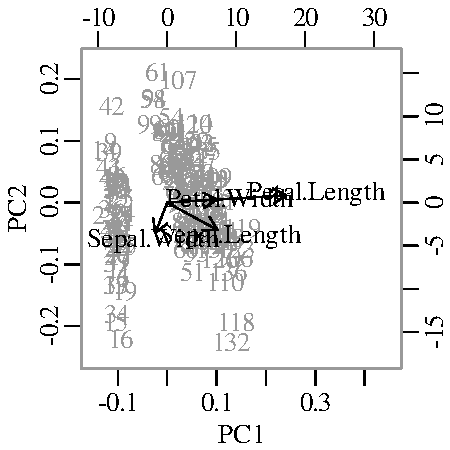
\includegraphics[width=\textwidth]{../figures/PCAiris.pdf}\\
\end{minipage}
\begin{minipage}[t][][t]{.65\indentwidth}
  \captionof{figure}{PCA biplot for the \texttt{iris} data. This
    diagram indicates there are two groups of flowers that with
    distinct petal width and length measurements (PC1).  Within these
    two groups, additional variability is caused by the sepal width
    and length (PC2). The vector loadings of the petal width and
    length point in the same direction, which means that these two
    variables are correlated with each other. The vector loading of
    the sepal width is perpendicular to that of the petal
    measurements, which means that the sepal and petal dimensions vary
    independently.\\}
  \label{fig:PCAiris}
\end{minipage}

\item Classical MDS analysis of the \texttt{iris} data:

\begin{script}
d <- dist(iris[,-5])
mds <- cmdscale(d)
plot(mds,type='n')
text(mds)
\end{script}

\noindent which produces essentially the same output as
Figure~\ref{fig:PCAiris} but without the arrows.

\item Repeating the code from
  Section~\ref{sec:R-unsupervised}.\ref{it:R-kmeans} for different
  numbers of clusters:

\begin{script}
K <- 10            # maximum number of clusters to evaluate
ss <- rep(0,K)     # initialise the vector with the sums of squares
for (k in 1:K){    # loop through all the k values
  fit <- kmeans(iris[,-5],centers=k) # fit the k means
  ss[k] <- fit$tot.withinss          # extract the sum of squares
}
plot(x=1:K,y=ss,type='b')            # plot as both lines and points
\end{script}

\noindent\begin{minipage}[t][][b]{.35\indentwidth}
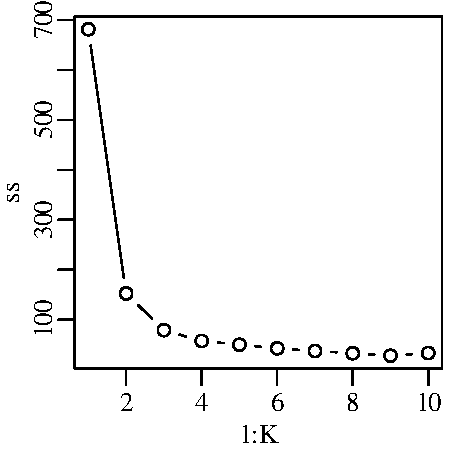
\includegraphics[width=\textwidth]{../figures/elbow.pdf}\\
\end{minipage}
\begin{minipage}[t][][t]{.65\indentwidth}
  \captionof{figure}{Evaluating the within-cluster sum-of-squares
    ($ss$) of the k-means algorithm for different numbers of clusters.
    The $ss$-misfit drops off very quicky before making an `elbow' at
    $k=3$ clusters. Hence we cannot justify more than 3 clusters.\\}
  \label{fig:elbow}
\end{minipage}

\item Using the \texttt{ksdist} function as instructed:

\begin{script}
data(DZ,package='geostats')
d <- ksdist(KS)
tree <- hclust(d)
plot(tree)
\end{script}

This produces the following tree:

\noindent\begin{minipage}[t][][b]{.35\indentwidth}
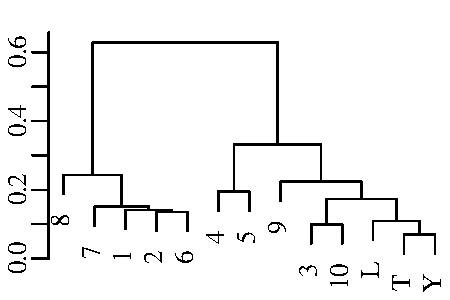
\includegraphics[width=\textwidth]{../figures/DZtree.pdf}\\
\end{minipage}
\begin{minipage}[t][][t]{.65\indentwidth}
  \captionof{figure}{Hierarchical clustering tree for the detrital
    zircon data. The tree conveys the same information as the MDS
    configuration of Figure~\ref{fig:DZmds}: there are two main
    clusters; T and Y are the two most similar samples; whilst L and 8
    are the two most dissimilar samples.}
  \label{fig:DZtree}
\end{minipage}

\end{enumerate}

\section{Supervised learning}
\label{sec:sol-supervised}

\begin{enumerate}

\item\label{it:sol-LDA-training} Build an LDA model for the
  \texttt{training} data:

\begin{script}
library(MASS)
data(training,package='geostats')
ld <- lda(affinity ~ ., data=training)
\end{script}

Predict the tectonic affinity of the \texttt{training} data:

\begin{script}[firstnumber=4]
pr <- predict(ld)
\end{script}

\noindent which is equivalent to:

\begin{script}[firstnumber=4]
pr <- predict(ld,newdata=training[,-1])
\end{script}

Count the number of misclassified \texttt{training} data:

\begin{console}
> sum(pr$class != training$affinity)
[1] 60
\end{console}

So 60 of the 646 training samples were misclassified (9\%).

\item\label{it:sol-LDA-test} Loading the \texttt{test} data into
  memory and classifying it with the \texttt{ld} model developed in
  answer~\ref{it:sol-LDA-training}:

\begin{script}
data(test,package='geostats')
pr.test <- predict(ld,newdata=test[,-1])
\end{script}

Count the number of misclassified \texttt{test} data:

\begin{console}
> sum(pr.test$class != test$affinity)
[1] 32
\end{console}

So 32 out of 147 of the \texttt{test} data were misclassified (21\%).
Unsurprisingly, this is higher than the misclassification rate of the
\texttt{training} data. Inspecting the results in some more detail:

\begin{console}
> table(pr.test$class,test$affinity)
       IAB MORB OIB
  IAB   48    2   1
  MORB  12   16   8
  OIB    4    5  51
\end{console}

This shows that the misclassification rates are similar for all three
tectonic affinities.

\item Repeating the code of exercise~\ref{it:sol-LDA-training} but
  replacing \texttt{MASS} with \texttt{rpart} and \texttt{lda} with
  \texttt{rpart}:
  
\begin{script}
library(rpart)
data(training,package='geostats')
tree <- rpart(affinity ~ ., data=training)
\end{script}

Predict the tectonic affinity of the \texttt{training} data:

\begin{script}[firstnumber=3]
pr <- predict(tree,type='class')
\end{script}

Count the number of misclassified \texttt{training} samples:

\begin{console}
> sum(pr != training$affinity)
[1] 42
\end{console}

So 42 of the 646 training samples were misclassified.

\item Repeating the code of exercise~\ref{it:sol-LDA-test} but
  replacing \texttt{MASS} with \texttt{rpart} and \texttt{lda} with
  \texttt{rpart}.
  
\begin{script}
data(test,package='geostats')
pr.test <- predict(tree,newdata=test[,-1],type='class')
\end{script}

Count the number of misclassified \texttt{test} data:

\begin{console}
> sum(pr.test != test$affinity)
[1] 28
\end{console}

So 28 out of 147 of the \texttt{test} data were misclassified (19\%).
Again, this is higher than the misclassification rate of the
\texttt{training} data, but slightly lower than the misclassification
rate of the \texttt{test} data by LDA.

\end{enumerate}

\section{Compositional data}
\label{sec:sol-compositional}

\begin{enumerate}
\item
  \begin{enumerate}
  \item\label{it:sol-mpg1} Calculate the arithmetic mean fuel
    consumption, in miles per gallon:

\begin{console}
> avg.mpg <- mean(mtcars[,'mpg'])
> avg.mpg
[1] 20.09062
\end{console}

\item\label{it:sol-mpg2} Convert the data to litres/100km:

\begin{console}
l100k <- 235/mtcars[,'mpg']
\end{console}

\item\label{it:sol-mpg3} Average the litres/100km:

\begin{console}
> avg.l100k <- mean(l100k)
> avg.l100k
[1] 12.7434
\end{console}

\item\label{it:sol-mpg4} Convert the arithmetic mean number of miles
  per gallon (from step~\ref{it:sol-mpg1}) to units of litre/100km.

\begin{console}
> avg.l100k.from.mpg <- 235/avg.mpg
> avg.l100k.from.mpg
[1] 11.697
\end{console}

\noindent which is \emph{not} equal to the 12.7434 litres/100km
obtained under step~\ref{it:sol-mpg3}. The difference is nearly 10\%.

\item\label{it:sol-mpg5} Compute the geometric mean fuel consumption
  in mpg and litres/100km, and convert the geometric mean mpg value to
  litres/100km:
  
\begin{console}
> geomean.mpg <- exp(mean(log(mtcars[,'mpg'])))
> geomean.l100k <- exp(mean(log(l100k)))
> geomean.l100k.from.mpg <- 235/geomean.mpg
> c(geomean.l100k,geomean.l100k.from.mpg)
[1] 12.20775 12.20775
\end{console}

\noindent which is an altogether more sensible result than that
obtained under step~\ref{it:sol-mpg4}.

\end{enumerate}

\item\label{it:sol-ternary-test} Load \texttt{geostats}' \texttt{test}
  data into memory and plot the
  CaO--K\textsubscript{2}O--Na\textsubscript{2}O subcomposition on a
  ternary diagram as filled grey circles:

\begin{script}
data(test,package='geostats')
alkali <- test[,c('CaO','K2O','Na2O')]
ternary(alkali,pch=16,col='grey50')
\end{script}

Adding the arithmetic mean as a white filled circle:

\begin{script}[firstnumber=4]
arithmetic.mean <- colMeans(alkali)
ternary(arithmetic.mean,add=TRUE,type='p',pch=21,bg='white')
\end{script}

Adding the logratio mean as a white filled square:

\begin{script}[firstnumber=6]
logratio.mean <- exp(colMeans(log(alkali)))
ternary(logratio.mean,add=TRUE,type='p',pch=22,bg='white')
\end{script}

\item PCA is an unsupervised learning technique. So we don't need to
  know the tectonic affinities, which are stored in the first column
  of the \texttt{training} data. Hence we split the \texttt{data} into
  two parts: the affinities and the data itself. The data is used for
  the PCA, and the affinities are used as labels to help us interpret
  the biplot:

\begin{script}
data(test,package='geostats')
aff <- test[,1]      # tectonic affinities
dat <- test[,-1]     # geochemical data
lrdat <- clr(dat)
pc <- prcomp(lrdat)
biplot(pc,col=c('grey50','black'),xlabs=aff)
\end{script}

\noindent\begin{minipage}[t][][b]{.5\indentwidth}
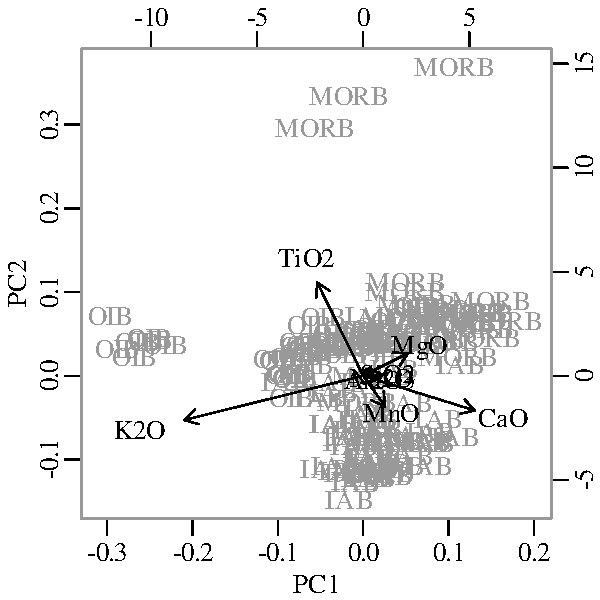
\includegraphics[width=\textwidth]{../figures/testPCA.pdf}\\
\end{minipage}
\begin{minipage}[t][][t]{.5\indentwidth}
  \captionof{figure}{PCA biplot of the oceanic basalt compositions.
    The data roughly fall into three clusters, corresponding to OIB,
    MORB and IAB. OIBs are relatively rich in K\textsubscript{2}O and
    poor in CaO; MORBs are rich in MgO and TiO\textsubscript{2}; and
    IABs are rich in MnO and poor in TiO\textsubscript{2}.
    K\textsubscript{2}O and CaO are anti-correlated, and so are
    TiO\textsubscript{2} and MnO. The variability in MnO/CaO is
    independent of the variability in TiO\textsubscript{2}/MnO.  The
    `outliers' on the ternary diagram of
    exercise~\ref{it:sol-ternary-test} are OIBs that are particularly
    poor in CaO.}
  \label{fig:testPCA}
\end{minipage}

\item Compositional LDA of the training data:

\begin{script}
data(training,package='geostats')
ld <- lda(x=alr(training[,-1]),grouping=training[,1])
pr.training <- predict(ld)
\end{script}

Compositional LDA of the test data:

\begin{script}[firstnumber=4]
data(test,package='geostats')
pr.test <- predict(ld,newdata=alr(test[,-1]))
\end{script}

Compare the fitted results with the true affinities:

\begin{console}
> sum(pr.training$class != training$affinity)
[1] 48
> sum(pr.test$class != test$affinity)
[1] 19
\end{console}

In contrast with the previous LDA results of
Section~\ref{sec:sol-supervised}.\ref{it:sol-LDA-training}--\ref{it:sol-LDA-test},
the logratio transformation has reduced the number of misclassified
samples from 60 to 48 for the training data, and from 32 to 19 for the
test data.

\end{enumerate}

\section{Directional data}
\label{sec:sol-directional}

\begin{enumerate}

\item Store the data into two variables:

\begin{script}
A <- c(50,55,40,60,45)
B <- c(350,10,5,358)
\end{script}

Then the difference of the vector means is given by

\begin{console}
> meanangle(A,degrees=TRUE) - meanangle(B,degrees=TRUE)
[1] 49.24496
\end{console}

(for comparison, the difference of the arithmetic means is
$-131^\circ$)

\item Load the earthquake data and extract the latitude and longitude
  values:

\begin{script}  
data(earthquakes,package='geostats')
lon <- earthquakes$lon
lat <- earthquakes$lat
\end{script}

Select the plottable longitudes and show on a Schmidt net:

\begin{script}[firstnumber=4]
good <- (lon>-90 & lon<90)
stereonet(trd=lon[good],plg=lat[good],option=3,degrees=TRUE,wulff=FALSE)
\end{script}

\item Store the data into two data frames:

\begin{script}
F1 <- data.frame(strike=c(200,195,210,205),dip=c(70,68,71,67))
F2 <- data.frame(strike=c(20,25,18,17,16),dip=c(10,12,9,14,11))
\end{script}

Plot the two sets of fault measurements on a single Wulff diagram (in
different colours to allow distinction):

\begin{script}[firstnumber=3]
stereonet(trd=F1$strike,plg=F1$dip,option=2,degrees=TRUE)
stereonet(trd=F2$strike,plg=F2$dip,option=2,degrees=TRUE,
          add=TRUE,col='grey')
\end{script}

Calculate the mean strike and dip:

\begin{script}[firstnumber=5]
mF1 <- meanangle(trd=F1$strike,plg=F1$dip,option=2,degrees=TRUE)
mF2 <- meanangle(trd=F2$strike,plg=F2$dip,option=2,degrees=TRUE)
\end{script}

Add these values to the existing stereoplot:

\begin{script}[firstnumber=5]
stereonet(trd=mF1[1],plg=mF1[2],option=2,degrees=TRUE,add=TRUE,pch=15)
stereonet(trd=mF2[1],plg=mF2[2],option=2,degrees=TRUE,add=TRUE,pch=15,
          col='grey')
\end{script}

Querying the mean vectors at the console:

\begin{console}
> mF1
[1] -157.67178   69.08943
> mF2
[1] 19.19848 11.21677
\end{console}

The difference between the strikes and dips is -176.9$^\circ$ and
57.9$^\circ$, respectively.

\item The same \texttt{Rbar} function that was used for the circular
  data in Section~\ref{sec:ex-directional}.\ref{it:Rbar} can also be
  used to calculating the concentration parameter ($\bar{R}$) of
  spherical data. For the \texttt{palaeomag} data:

\begin{console}  
> Rbar(trd=palaeomag$decl,plg=palaeomag$incl,option=1,degrees=TRUE)
[1] 0.9927666
\end{console}

\noindent and for the \texttt{fault} data:

\begin{console}  
> Rbar(trd=fault$strike,plg=fault$dip,option=2,degrees=TRUE)
[1] 0.9970092
\end{console}

Because the latter value is higher than the former, we conclude that
the fault orientation data are more strongly concentrated than the
palaeomagnetic data.

\end{enumerate}

\section{Spatial data}
\label{sec:sol-spatial}

\begin{enumerate}
  
\item\label{it:normodel} Load the \texttt{hills} dataset and storing
  the three columns in separate variables for brevity:

\begin{script}
data(hills,package='geostats')
X <- hills$X
Y <- hills$Y
Z <- hills$Z
\end{script}

Fit the four semivariogram models:

\begin{script}[firstnumber=5]
par(mfrow=c(2,2))
normodel <- semivariogram(x=X,y=Y,z=Z,plot=TRUE,model='gaussian')
expmodel <- semivariogram(x=X,y=Y,z=Z,plot=TRUE,model='exponential')
linmodel <- semivariogram(x=X,y=Y,z=Z,plot=TRUE,model='linear')
sphmodel <- semivariogram(x=X,y=Y,z=Z,plot=TRUE,model='spherical')
\end{script}

Visual inspection of the resulting plots indicates that the Gaussian
model fits the empirical semivariogram best, which is not surprising
given that the \texttt{hills} dataset consists of a bivariate Gaussian
mixture.

\noindent\begin{minipage}[t][][b]{\indentwidth}
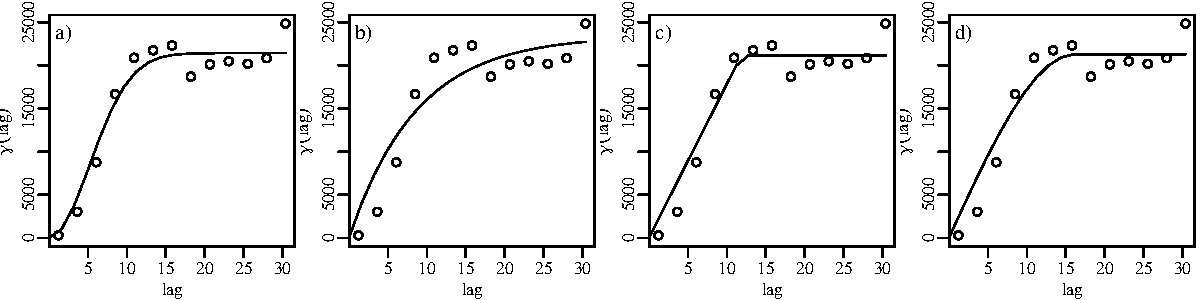
\includegraphics[width=\indentwidth]{../figures/hills.pdf}
\end{minipage}
\begin{minipage}[t][][t]{\indentwidth}
\captionof{figure}{a) Gaussian; b) exponential; c) linear and d)
  spherical semivariogram fits to the \texttt{hills} data.}
\end{minipage}

\item Kriging interpolation of $\{x=0,y=0\}$ using the
  \texttt{normodel} semivariogram model from step~\ref{it:normodel}:

\begin{console}
> kriging(x=X,y=Y,z=Z,xi=0,yi=0,svm=normodel)
[1] 538.1133
\end{console}

\noindent and the standard error:

\begin{console}
> v <- kriging(x=X,y=Y,z=Z,xi=0,yi=0,svm=normodel,err=TRUE)
> sqrt(v)
[1] 6.180623
\end{console}

Hence the elevation estimate at $\{x=0,y=0\}$ is $538 \pm 6$~m.

\item Following the numerical recipe of
  Section~\ref{sec:R-spatial}.\ref{it:R-meuse-contour}:

\begin{script}[firstnumber=11]
xi <- seq(from=min(X),to=max(X),length.out=30)
yi <- seq(from=min(Y),to=max(Y),length.out=30)
zi <- kriging(x=X,y=Y,z=Z,xi=xi,yi=yi,svm=normodel,grid=TRUE)
colourplot(x=xi,y=yi,z=zi,colspec=grey)
\end{script}

\item Fitting spherical and exponential semivariogram models to the
  Meuse data:

\begin{script}
data(meuse,package='geostats')
X <- meuse$x
Y <- meuse$y
Z <- log(meuse$zinc)
sphmodel <- semivariogram(x=X,y=Y,z=Z,plot=FALSE,model='spherical')
expmodel <- semivariogram(x=X,y=Y,z=Z,plot=FALSE,model='exponential')
\end{script}

Estimating the log[Zn] values along an $x-y$ grids for both models:

\begin{script}[firstnumber=7]
xi <- seq(from=min(X),to=max(X),length.out=50)
yi <- seq(from=min(Y),to=max(Y),length.out=50)
zsph <- kriging(x=X,y=Y,z=Z,xi=xi,yi=yi,grid=TRUE,svm=sphmodel)
zexp <- kriging(x=X,y=Y,z=Z,xi=xi,yi=yi,grid=TRUE,svm=expmodel)
colourplot(x=xi,y=yi,z=zsph-zexp,colspec=grey)
\end{script}

The largest disagreements are found in sparsely sampled parts of the
map. To show the sample locations as white circles, use the
\texttt{colourplots}'s optional \texttt{extra} argument:

\begin{script}[firstnumber=11]
colourplot(x=xi,y=yi,z=exp(zsph-zexp),colspec=grey,
           extra={points(X,Y,pch=16,col='white')})
\end{script}

\noindent which also exponentiates the log-contrasts to yield the
ratio of the Zn-concentation estimate using the spherical and
exponential semivariogram models.

\noindent\begin{minipage}[t][][b]{.6\indentwidth}
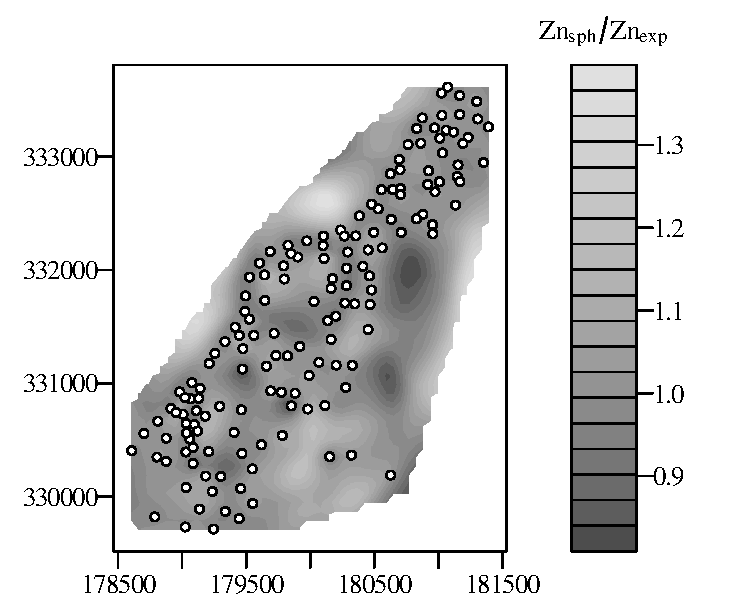
\includegraphics[width=\textwidth]{../figures/sphvsexp.pdf}
\end{minipage}
\begin{minipage}[t][][t]{.4\indentwidth}
  \captionof{figure}{Log-contrast between two kriging interpolations
    for the Meuse data, using the spherical and exponential
    semivariogram models. The 155 measurements locations are marked by
    white circles. The smallest discrepancies ($<10\%$) are found in
    densely sampled areas. In more sparsely sampled parts of the
    contour plot, and especially near the edges, the disagreement
    between the spherical and exponential models increases to up to
    $60\%$.}
\end{minipage}

\end{enumerate}
